\documentclass[aspectratio=169]{beamer}

\graphicspath{{graphics/}}

\usetheme[style=fwn]{leidenuniv}
\useinnertheme{circles}
\useoutertheme[subsection=false]{miniframes}
\beamertemplatenavigationsymbolsempty

\usepackage{booktabs}
\usepackage[style=verbose,backend=biber]{biblatex}
\addbibresource{../snacspaper.bib}

% uncomment next line to let framesubtitle have palette primary color
%\setbeamercolor{framesubtitle}{use={palette primary},fg=palette primary.bg}

% uncomment next line to remove navigation symbols from the pdf
%\setbeamertemplate{navigation symbols}{}

\title{node2vec: Scalable Feature Learning for Networks}
\subtitle{Authors: Aditya Grover and Jure Leskovec}
\author{Chenyu Shi and Shupei Li}
\institute[LIACS]{Leiden Institute of Advanced Computer Science}
\date{November 18, 2022}


\begin{document}

\begin{frame}[plain]
	\titlepage
\end{frame}

\begin{frame}
	\tableofcontents
\end{frame}

\section{Introduction}
\begin{frame}
    \frametitle{Introduction to Graph Embeddings}
    \begin{itemize}
        \item Represent graph-structured data.
        \item Applications: \\
            Social network analysis, recommender systems, molecular structure modelling, etc.
        \item Challenge: Limitations of traditional methods.
        \item Development of techniques specially for graph representations.
    \end{itemize}
\end{frame}

\section{Related Work}
\begin{frame}
    \frametitle{Related Work}
    A taxonomy of graph embedding techniques \footcite{murphy2022}.
    \begin{center}
        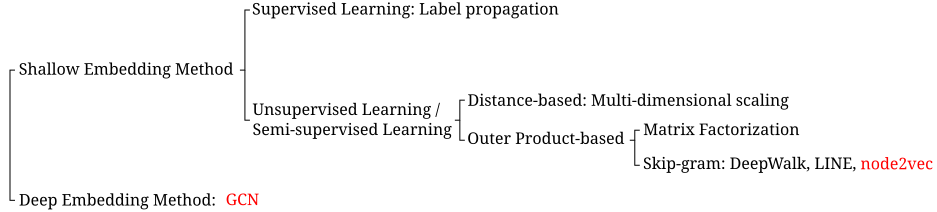
\includegraphics[width=14cm]{./graphics/related-work.png}
    \end{center}
\end{frame}

\section{Methodology}
\begin{frame}
    
\end{frame}

\section{Experiments}
\begin{frame}
    \frametitle{Experiment 1: Multi-label Classification}
    \begin{itemize}
        \item Task description
            \begin{itemize}
                \item[$\circ$] Labels from a finite set $\mathcal{L}$
                \item[$\circ$] Training: A fraction of nodes and all their labels.
                \item[$\circ$] Predict the labels for the remaining nodes.
            \end{itemize}
        \item Data\par
            ~\\
            \begin{tabular}{llll}
                \toprule
                \textbf{Dataset} & \textbf{Nodes} & \textbf{Edges} & \textbf{Labels}\\
                \midrule
                BlogCatalog & 10,312 & 333,983 & 39\\
                Protein-Protein Interactions (PPI) & 3,890 & 76,584 & 50\\
                Wikipedia & 4,777 & 184,812 & 40\\
                \bottomrule
            \end{tabular}
    \end{itemize}
\end{frame}

\begin{frame}
    \frametitle{Experiment 1: Multi-label Classification}
    \begin{itemize}
        \item Results\par
            ~\\
            \begin{tabular}{llll}
                \toprule
                \textbf{Algorithm} & & \textbf{Dataset} &\\
                             & BlogCatalog & PPI & Wikipedia\\
                \midrule
                Spectral Clustering & 0.0405 & 0.0681 & 0.0395\\
                DeepWalk & 0.2110 & 0.1768 & 0.1274\\
                LINE & 0.0784 & 0.1447 & 0.1164\\
                node2vc & \textbf{0.2581} & \textbf{0.1791} & \textbf{0.1552}\\
                \midrule
                node2vec settings (p, q) & 0.25, 0.25 & 4, 1 & 4, 0.5\\
                Gain of node2vec [\%] & \textbf{22.3} & \textbf{1.3} & \textbf{21.8}\\
                \bottomrule
            \end{tabular}
    \end{itemize}
\end{frame}

\begin{frame}
    \frametitle{Experiment 2: Link Prediction}
    \begin{itemize}
        \item Task description
            \begin{itemize}
                \item[$\circ$] A network with a fraction of edges removed.
                \item[$\circ$] Predict these missing edges.
            \end{itemize}
        \item Data\par
            ~\\
            \begin{tabular}{lll}
                \toprule
                \textbf{Dataset} & \textbf{Nodes} & \textbf{Edges}\\
                \midrule
                Facebook & 4,039 & 88,234 \\
                Protein-Protein Interactions (PPI) & 19,706 & 390,633\\
                arXiv ASTRO-PH & 18,722 & 198,110\\
                \bottomrule
            \end{tabular}
    \end{itemize}
\end{frame}

\begin{frame}
    \frametitle{Experiment 2: Link Prediction}
    \begin{itemize}
        \item Results\par
            ~\\
            \begin{tabular}{llll}
                \toprule
                \textbf{Algorithm} & & \textbf{Dataset} & \\
                             & Facebook & PPI & arXiv \\
                \midrule
                Common Neighbors & 0.8100 & 0.7142 & 0.8153\\
                Jaccard's Coefficient & 0.8880 & 0.7018 & 0.8067\\
                Adamic-Adar & 0.8289 & 0.7126 & 0.8315\\
                Pref. Attachment & 0.7137 & 0.6670 & 0.6996\\
                Spectral Clustering & 0.6192 & 0.4920 & 0.5740\\
                DeepWalk & \textbf{0.9680} & 0.7441 & 0.9340\\
                LINE & 0.9490 & 0.7249 & 0.8902\\
                mode2vec & \textbf{0.9680} & \textbf{0.7719} & \textbf{0.9366}\\
                \bottomrule
            \end{tabular}
    \end{itemize}
\end{frame}

\begin{frame}
    
\end{frame}

\section{Our work}
\begin{frame}
    \frametitle{Preliminary Results}
\end{frame}

\section{Future work}
\begin{frame}
    \frametitle{Future work} 
\end{frame}

\end{document}
